\chapter{Introduction to Triangles}

Connecting any three points with three line segments will get you a
triangle. Here is the triangle $ABC$, which was created by connecting three points $A$, $B$, and $C$:\index{triangle}

\begin{tikzpicture}[scale=1.5]
  \coordinate [circle, fill, inner sep=2pt] (a) at (0,0) ;
  \coordinate [circle, fill, inner sep=2pt] (b) at (1, 2) ;
  \coordinate [circle, fill, inner sep=2pt] (c) at (3,0) ;
  \draw (a)--(b) node [outer sep=3pt, above]{$B$};
  \draw (b)--(c) node[outer sep=3pt, right]{$C$};
  \draw (c)--(a) node[outer sep=3pt, left]{$A$};
\end{tikzpicture}

\section{Equilateral and Isosceles Triangles}
% Add scalene Triaganle
We talk a great deal about the length of the sides of triangles. If all three sides of the triangle are the same length, we say it is an \emph{equilateral triangle}:\index{equilateral triangle}

\begin{tikzpicture}[scale=1.5]
  \coordinate [circle, fill, inner sep=2pt] (a) at (0,0) ;
  \coordinate [circle, fill, inner sep=2pt] (b) at (1.5, 2.6) ;
  \coordinate [circle, fill, inner sep=2pt] (c) at (3,0) ;
  \draw (a)--(b) node [outer sep=3pt, above]{$B$};
  \draw (b)--(c) node[outer sep=3pt, right]{$C$};
  \draw (c)--(a) node[outer sep=3pt, left]{$A$};
  \tkzMarkSegment[pos=.5,mark=||](a,b)
  \tkzMarkSegment[pos=.5,mark=||](b,c)
  \tkzMarkSegment[pos=.5,mark=||](c,a)
\end{tikzpicture}

If only two sides of the triangle are the same length, we say it is an \emph{isosceles triangle}:\index{isoscelese triangle}

\begin{tikzpicture}[scale=1.3]
  \coordinate [circle, fill, inner sep=2pt] (a) at (0,0) ;
  \coordinate [circle, fill, inner sep=2pt] (b) at (1.5, 4) ;
  \coordinate [circle, fill, inner sep=2pt] (c) at (3,0) ;
  \draw (a)--(b) node [outer sep=3pt, above]{$B$};
  \draw (b)--(c) node[outer sep=3pt, right]{$C$};
  \draw (c)--(a) node[outer sep=3pt, left]{$A$};
  \tkzMarkSegment[pos=.5,mark=||](a,b)
  \tkzMarkSegment[pos=.5,mark=||](c,b)
\end{tikzpicture}

The shortest distance between two points is always the straight line
between them. This means you can be certain that the length of one side
will \emph{always} be less than the sum of the lengths of the
remaining two sides. This is known as the \emph{triangle inequality}.\index{triangle inequality}

For example, in this diagram, $c$ must be less than $a + b$.

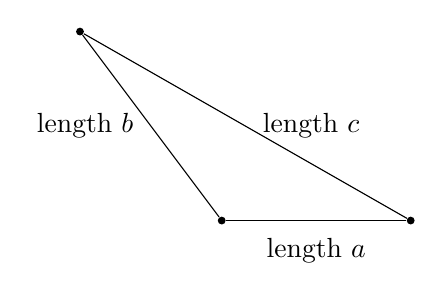
\begin{tikzpicture}[scale=1.2]
  \coordinate [circle, fill, inner sep=1pt] (a) at (1.5,0) ;
  \coordinate [circle, fill, inner sep=1pt] (b) at (0,2) ;
  \coordinate [circle, fill, inner sep=1pt] (c) at (3.5,0) ;
  \draw (a)--node[outer sep=3pt, left]{length $b$}(b) ;
  \draw (b)--node[outer sep=3pt, right]{length $c$}(c) ;
  \draw (c)--node[outer sep=3pt, below]{length $a$}(a) ;
\end{tikzpicture}

\section{Interior Angles of a Triangle}

We also talk a lot about the interior angles of a triangle:

\begin{tikzpicture}[scale=2]
  \coordinate [circle, fill, inner sep=2pt] (a) at (0,0) ;
  \coordinate [circle, fill, inner sep=2pt] (b) at (1, 2) ;
  \coordinate [circle, fill, inner sep=2pt] (c) at (3,0) ;
  \draw (a)--(b) node [outer sep=3pt, above]{$B$};
  \draw (b)--(c) node[outer sep=3pt, right]{$C$};
  \draw (c)--(a) node[outer sep=3pt, left]{$A$};
  \pic [draw, <->, "$a$", angle eccentricity=1.5] {angle = c--a--b};
  \pic [draw, <->, "$b$", angle eccentricity=1.5] {angle = a--b--c};
  \pic [draw, <->, "$c$", angle eccentricity=1.5] {angle = b--c--a};
\end{tikzpicture}

A triangle where one of the interior angles is a right angle is said to be a \emph{right triangle}:\index{right triangle}

\begin{tikzpicture}[scale=1.2]
  \coordinate [circle, fill, inner sep=2pt] (a) at (0,0) ;
  \coordinate [circle, fill, inner sep=2pt] (b) at (0,4) ;
  \coordinate [circle, fill, inner sep=2pt] (c) at (3,0) ;
  \draw (a)--(b) node [outer sep=3pt, above]{$B$};
  \draw (b)--(c) node[outer sep=3pt, right]{$C$};
  \draw (c)--(a) node[outer sep=3pt, left]{$A$};
  \pic [draw,angle eccentricity=1.5] {right angle = c--a--b};
\end{tikzpicture}

If a triangle has an obtuse interior angle, it is said to be an \emph{obtuse triangle}:\index{obtuse triange}

\begin{tikzpicture}[scale=1.2]
  \coordinate [circle, fill, inner sep=2pt] (a) at (1.5,0) ;
  \coordinate [circle, fill, inner sep=2pt] (b) at (0,2) ;
  \coordinate [circle, fill, inner sep=2pt] (c) at (3.5,0) ;
  \draw (a)--(b) node [outer sep=3pt, above]{$B$};
  \draw (b)--(c) node[outer sep=3pt, right]{$C$};
  \draw (c)--(a) node[outer sep=3pt, left]{$A$};
  \pic [draw, <->, "obtuse", angle eccentricity=1.7] {angle = c--a--b};
\end{tikzpicture}

If all three interior angles of a triangle are less than $90^\circ$, it is said to be an \emph{acute triangle}.\index{acute triangle}

The measures of the interior angles of a triangle always add up to
$180^\circ$. For example, if we know that a triangle has interior
angles of $37^\circ$ and $56^\circ$, we know that the third
interior angle is $87^\circ$.

\begin{Exercise}[title={Missing Angle}, label=missing_angle]
One interior angle of a triangle is $92^\circ$. The second angle is $42^\circ$. What is the measure of the third interior angle?
\end{Exercise}
\begin{Answer}[ref=missing_angle]
$180^\circ - (92^\circ + 42^\circ) = 46^\circ$
\end{Answer}

% Needs Diagram
How can you know that the sum of the interior angles is $180^\circ$?
Imagine that you started on the edge of a triangle and walked all the
way around to where you started. ( going
counter-clockwise.) You would turn three times to the left:

\begin{tikzpicture}[scale=1.7]
  \coordinate [circle, fill, inner sep=2pt] (a) at (1.5,0) ;  
   \node at (a) [outer sep=3pt, left]{$A$};
  \coordinate [circle, fill, inner sep=2pt] (b) at (0.5,2) ;
  \node at (b) [outer sep=3pt, above]{$B$} ;
  \coordinate [circle, fill, inner sep=2pt] (c) at (3.5,0) ;
    \node at (c)[outer sep=3pt, below]{$C$};
    
    \coordinate [circle, fill, inner sep=2pt](start) at (2.75,0);
    \node at (start)[outer sep=3pt, below]{Start};

   \coordinate (aa) at (1.75,-0.5) ;  
  \coordinate (bb) at (-0.25,2.5) ;
  \coordinate (cc) at (4.2,0) ;
  \draw [->](a)--(cc);
  \draw [->](b)--(aa);
  \draw [->](c)--(bb);
  \pic [draw, ->, "$T_C$", angle eccentricity=1.7] {angle = cc--c--b};
  \pic [draw, ->, "$T_B$", angle eccentricity=2] {angle = bb--b--a};
  \pic [draw, ->, "$T_A$", angle eccentricity=2] {angle = aa--a--c};
\end{tikzpicture}

After these three turns, you would be facing the same direction that
you started in. Thus, $T_A + T_B + T_C = 360^\circ$. The
measures of the interior angles are $a$, $b$, and $c$. Notice that $a$ and
$T_A$ are supplementary. So we know that:
\begin{itemize}
\item $T_A = 180 - a$
\item $T_B = 180 - b$
\item $T_C = 180 - c$
\end{itemize}
So we can rewrite the equation above as
\begin{equation*}
  (180 - a) + (180 - b) + (180 - c) = 360^\circ
\end{equation*}
Which is equivalent to
\begin{equation*}
  a + b + c = 360^\circ
\end{equation*}

\begin{Exercise}[title={Interior Angles of a Quadrilateral}, label=interior_of_quad]
  Any four-sided polygon is a \emph{quadrilateral}. Using the same
  ``walk around the edge'' logic, what is the sum of the interior
  angles of any quadrilateral?
\end{Exercise}
\begin{Answer}[ref=interior_of_quad]
$360^\circ$
\end{Answer}

